\documentclass[]{article}

% Imported Packages
%------------------------------------------------------------------------------
\usepackage{amssymb}
\usepackage{amstext}
\usepackage{amsthm}
\usepackage{amsmath}
\usepackage{enumerate}
\usepackage{fancyhdr}
\usepackage[margin=1in]{geometry}
\usepackage{graphicx}
%\usepackage{extarrows}
%\usepackage{setspace}
%------------------------------------------------------------------------------

% Header and Footer
%------------------------------------------------------------------------------
\pagestyle{plain}  
\renewcommand\headrulewidth{0.4pt}                                      
\renewcommand\footrulewidth{0.4pt}                                    
%------------------------------------------------------------------------------

% Title Details
%------------------------------------------------------------------------------
\title{Deliverable \#2 Template}
\author{SE 3A04: Software Design II -- Large System Design}
\date{}                               
%------------------------------------------------------------------------------

% Document
%------------------------------------------------------------------------------
\begin{document}

\maketitle	
\noindent{\bf Tutorial Number:} T03\\
{\bf Group Number:} G07 \\
{\bf Group Members:} 
\begin{itemize}
	\item Farid Bastoros 
	\item Neha Bhatla
	\item Omar Alam
	\item Luka Mahrt-Smith
	\item Aidan Lao
\end{itemize}

\section*{IMPORTANT NOTES}
\begin{itemize}
	%	\item You do \underline{NOT} need to provide a text explanation of each diagram; the diagram should speak for itself
	\item Please document any non-standard notations that you may have used
	\begin{itemize}
		\item \emph{Rule of Thumb}: if you feel there is any doubt surrounding the meaning of your notations, document them
	\end{itemize}
	\item Some diagrams may be difficult to fit into one page
	\begin{itemize}
		\item Ensure that the text is readable when printed, or when viewed at 100\% on a regular laptop-sized screen.
		\item If you need to break a diagram onto multiple pages, please adopt a system of doing so and thoroughly explain how it can be reconnected from one page to the next; if you are unsure about this, please ask about it
	\end{itemize}
	\item Please submit the latest version of Deliverable 1 with Deliverable 2
	\begin{itemize}
		\item Indicate any changes you made.
	\end{itemize}
	\item If you do \underline{NOT} have a Division of Labour sheet, your deliverable will \underline{NOT} be marked
\end{itemize}

\newpage
\section{Introduction}
\label{sec:introduction}
% Begin Section

This section should provide an brief overview of the entire document.

\subsection{Purpose}
\label{sub:purpose}
% Begin SubSection
This document provides a high-level overview of the Shroomify system architecture, outlining the core design principles, subsystems, and the rationale behind architectural choices. It is intended for internal stakeholders involved in the development of Shroomify, including software engineers, project managers, investors, domain experts, and system architects. Prior technical knowledge is beneficial but not required for understanding this document. 
% End SubSection

\subsection{System Description}
\label{sub:system_description}
% Begin SubSection
Give a brief description of the system. This could be a paragraph or two to give some context to this document.

% End SubSection

\subsection{Overview}
\label{sub:overview}
% Begin SubSection
This is Deliverable 2 of the Shroomify project and provides a general description of the system architecture. It considers the requirements, use cases, and design decisions outlined in Deliverable 1. Section 2 has an Analysis Class Diagram that represents the major classes and how they relate to each other from our requirements analysis. This diagram establishes the foundation for the organization of the system internally and ensures that design is high in cohesion and low in coupling among its components. Section 3 presents a description of the Architectural Design of Shroomify. In this section, we define the chosen architectural pattern and discuss specific design decisions. Section 4 focused on Class Responsibility Collaboration (CRC) Cards. These cards capture the responsibilities and communications of each class within the system, detailing exactly how the individual components interact to satisfy the demands of the system.

% End SubSection

% End Section
\clearpage
\section{Analysis Class Diagram}
\label{sec:analysis_class_diagram}
% Begin Section
This section should provide an analysis class diagram for your application.
\begin{figure}[h]
    \centering
    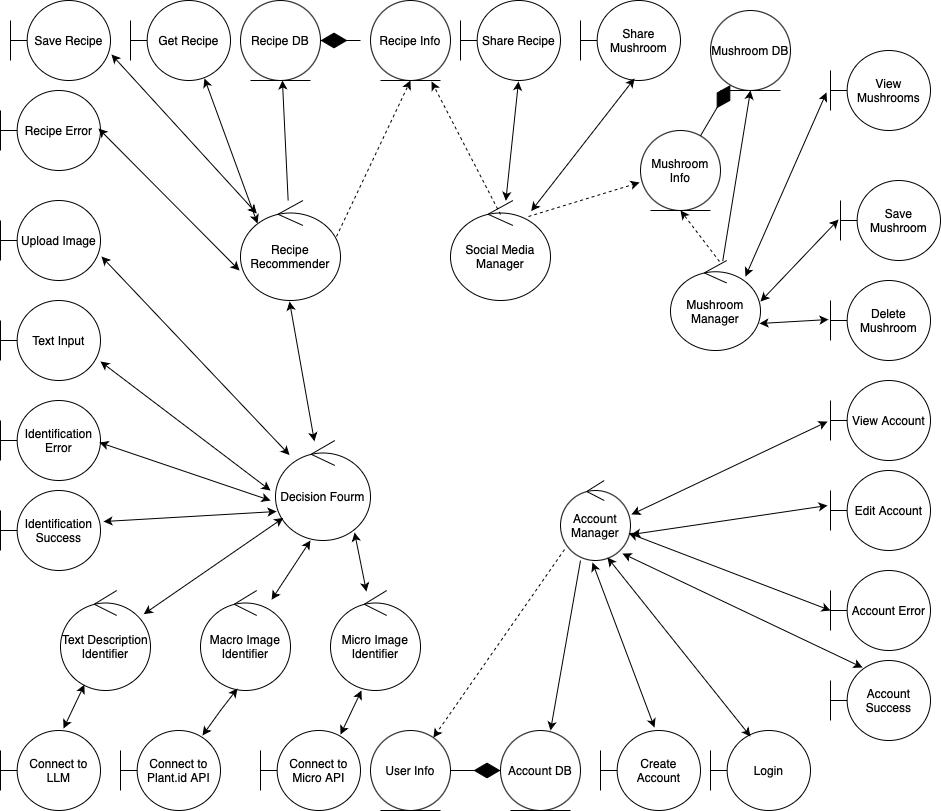
\includegraphics[width=1\textwidth]{AnalysisClassDiagram.png}
    \caption{Analysis Class Diagram}
    \label{fig:sample}
\end{figure}
% End Section

\clearpage
\section{Architectural Design}
\label{sec:architectural_design}
% Begin Section
This section should provide an overview of the overall architectural design of your application. Your overall architecture should show the division of the system into subsystems with high cohesion and low coupling.

\subsection{System Architecture}
\label{sub:system_architecture}
% Begin SubSection
\begin{itemize}
	\item Identify and explain the overall architecture of your system
	\item Be sure to clearly state the name of the architecture you used (this is the name of the architectural pattern, not the name of your system)
	\item Provide the reasoning and justification of the choice of architecture
	\item Provide a structural architecture diagram showing the relationship among the subsystems (if appropriate)
	\item List any design alternatives you considered, but eliminated (and explain why you eliminated them)
\end{itemize}
% End SubSection

\subsection{Subsystems}
\label{sub:subsystems}
% Begin SubSection
\subsubsection{Subsystem Overview}
Our system is divided into five main subsystems: \textbf{Decision Forum, Mushroom Management, Account Management, Social Media Management, and Recipe Recommendation}. These subsystems interact to provide users with a seamless experience in identifying mushrooms, managing their findings, and sharing information.

\subsubsection{Decision Forum}
The \textbf{Decision Forum} subsystem is responsible for identifying mushrooms. It contains the \textbf{machine learning algorithm} that classifies mushrooms based on user-provided descriptions and \textbf{computer vision technology} that analyzes images to determine species. If the identification confidence is low, users can also post images and descriptions to receive verification from the community.

\paragraph{Purpose}
Automates mushroom identification using AI and provides a space for community-based verification.

\paragraph{Relationship to Other Subsystems}
\begin{itemize}
    \item Works with \textbf{Mushroom Management} to store confirmed identifications.
    \item Interfaces with \textbf{Account Management} to associate identifications with users.
    \item Can interact with \textbf{Social Media Management} for users to share identification discussions.
\end{itemize}

\subsubsection{Mushroom Management}
The \textbf{Mushroom Management} subsystem serves as a \textbf{personal dictionary} of previously identified mushrooms. It allows users to view mushrooms they’ve found in the past, track their quantity, and access relevant information, including images and descriptions.

\paragraph{Purpose}
Stores and displays user-identified mushrooms but does \textbf{not} perform identification itself.

\paragraph{Relationship to Other Subsystems}
\begin{itemize}
    \item Retrieves identification results from \textbf{Decision Forum} and saves them.
    \item Integrates with \textbf{Account Management} to store mushroom data within user profiles.
    \item Interfaces with \textbf{Recipe Recommendation} to provide relevant recipes for identified mushrooms.
\end{itemize}

\subsubsection{Account Management}
The \textbf{Account Management} subsystem handles user authentication, profile settings, and data storage. It maintains a personalized record of identified mushrooms and user activity.

\paragraph{Purpose}
